% --------------------------------------------------------------------
% Technical Documentation
% Marco Müller
% --------------------------------------------------------------------

\documentclass[11pt, a4paper, listof=numbered, captions=tableheading, headinclude, table, xcdraw]{scrreprt}

\usepackage[utf8]{inputenc}
\usepackage[ngerman]{babel}
\usepackage{tikz}
\usepackage{epigraph}
%\usepackage[T1]{fontenc}
\usepackage{amsmath}
\usepackage{textgreek}
\usepackage[LGRgreek]{mathastext}
\usepackage{array}
\usepackage{color}
\usepackage{graphicx}
\usepackage{float}
\usepackage{helvet}
\usepackage{scrhack}
\renewcommand{\familydefault}{\sfdefault}

\setlength{\emergencystretch}{\hsize}
%\tolerance=9999

\newcounter{divide}

% für referenziertes Inhaltsverzeichnis
\usepackage[hidelinks, hypertexnames=false]{hyperref}

\usepackage{chngcntr}
\counterwithin*{chapter}{divide}

\renewcommand\epigraphflush{flushright}
\renewcommand\epigraphsize{\normalsize}
\setlength\epigraphwidth{0.7\textwidth}

\definecolor{titlepagecolor1}{cmyk}{1,.39,.0,.27}
\definecolor{titlepagecolor}{cmyk}{0,.82,.78,.30}

\DeclareFixedFont{\titlefont}{T1}{ppl}{b}{it}{0.5in}

\setlength{\parindent}{0pt}


% Seitenränder festlegen
\usepackage[top=1.5cm,bottom=1.5cm, includeheadfoot]{geometry}

% Blindtext für Testzwecke
%\usepackage{blindtext}
%\usepackage{lipsum}

% ---------------------------------------
% Titeldefinition
\newcommand{\Titel}{Dokumentation\\\vspace{.5mm}SynPLC}
\newcommand{\Caption}{Eine Selbstbau-SPS (oder so ähnlich)}
\newcommand{\SignateAuthor}{\textit{Erstellt mit \LaTeX}}
\newcommand{\Stand}{\textit{Stand: \today}}
% Sonstiges in titel.ltx und titel-meta.ltx
% ---------------------------------------

% Kopf- und Fußzeile
\usepackage[automark]{scrlayer-scrpage}



% --------------------------------------------------------------------
% Titelblatt
% --------------------------------------------------------------------

\input{titel/titel-meta.tex}
\begin{document}
\input{titel/titel.tex}


% --------------------------------------------------------------------
% Verzeichnisse
% --------------------------------------------------------------------

\pagenumbering{Roman}
\renewcommand{\thechapter}{\Roman{chapter}}

\setcounter{tocdepth}{2} %Ausblenden von Subsections etc..
\cohead[I. Inhaltsverzeichnis]{I. Inhaltsverzeichnis}
\pagestyle{scrheadings}
\tableofcontents 	\newpage
\cohead[II. Tabellenverzeichnis]{II. Tabellenverzeichnis}
\pagestyle{scrheadings}
\listoffigures 		\newpage
\cohead[III. Abbildungsverzeichnis]{III. Abbildungsverzeichnis}
\pagestyle{scrheadings}
\listoftables 		\newpage
\pagenumbering{arabic}

\stepcounter{divide}

\renewcommand{\thechapter}{\arabic{chapter}}

% Kopfzeilen erst nach den Verzeichnissen

\lohead[\today]{\today}
\cohead[ModLab V1.0]{ModLab V1.0}
\rohead[Marco Müller]{Marco Müller}
\pagestyle{scrheadings}

% --------------------------------------------------------------------
% Ab hier der Inhalt
% --------------------------------------------------------------------

\chapter{Vorwort}
Die SynPLC ist eine Selbstbau-SPS, die nach und nach entwickelt und verfeinert wird. 

Folgende Module sind in V1.0 vorhanden: 
\begin{itemize}
    \item CPU-Modul
    \item DO-Modul
    \item DI-Modul
    \item AO-Modul
\end{itemize}

Folgende Module befinden sich in Planung:
\begin{itemize}
    \item AI-Modul
    \item Interface-Modul
    \item Phasenanschnittmodul
\end{itemize} 			\newpage 	% Vorwort
\chapter{Bus-Systeme}
Die CPU V1.0 unterstützt nativ zwei Bus-Physiken:
\begin{enumerate}
    \item RS485
    \item CAN
\end{enumerate}

Für die IO-Module V1 wird nur RS485 unterstützt. Dazu wird auf der CPU die Steckbrücke für den Backplane entsprechend gesetzt.

\section{RS485}
Der RS485-Bus ist für die IO-Module der V1 vorgesehen. Dieser ist einfach auch auf kleineren und günstigeren Controllern zu nutzen und bietet genug Sicherheit über längere Strecken durch seinen differentiellen Aufbau.

Ursprünglich war angedacht, hier das ModBus RTU Protokoll zu nutzen, allerdings wurde dagegen entschieden und ein eigenes Protokoll entwickelt, was direkter ist und einige Funktionen mehr unterstützt. Auch sind die Funktionen auf die IO-Module zurechtgeschnitten.

\subsection{Adressen}
Es wird ein 8-bit Adressverfahren genutzt. Dies passt in die seriellen Buffer der Controller. Außerdem ist nicht vorgesehen, mehr als 32 Geräte eines Typs gleichzeitig zu benutzen. Damit die CPU von sich aus weiß, welches Modul auf welcher Adresse ist, sind die Adressen kodiert. 

\begin{table}[h]
    \centering
\begin{tabular}{|c|c|}
    \hline
    Modul       &       Adressbereich \\ \hline \hline
    CPU         &   111X XXXX \\ \hline
    Inferface   &   001X XXXX \\ \hline
    Digital Out &   010X XXXX \\ \hline
    Digital In  &   011X XXXX \\ \hline
    Analog Out  &   100X XXXX \\ \hline
    Analog In   &   101X XXXX \\ \hline
    PWM         &   110X XXXX \\ \hline
\end{tabular}
\caption{Adressen RS485}
\label{tab:Adressen RS485}
\end{table}

\newpage
\subsection{Protokoll}
Das Protokoll, welches über die RS485-Physik geht, ist relativ einfach, aber praktisch aufgebaut. Es bietet die Möglichkeit, den Bus u scannen um zu schauen, ob alle vorgegebenen Teilnehmer vorhanden sind, sowie Daten zu lesen und zu schreiben. Betrieben wird der Bus auf 250.000 Baud.

Aufgebaut ist es wie ein Multi-Master Bus, bei dem allerdings die CPU das ganze organisiert. Die eingebetteten Funktionen sind im Nachfolgenden einzeln erklärt.

Dabei ist zu bedenken, dass alle Befehle in den Slaves Register schreiben. Die Register werden nach dem Datentransfer in den Slaves ausgelesen und entsprechend verarbeitet. Eine Register-Map liegt jedem Modul der V1 bei.

\subsubsection{Scan/Ping}
Um zu schauen, ob ein Teilnehmer auf einer Adresse allgemein anwesend ist, kann man den Ping-Command senden. Dieser dient auch dazu, am Anfang den Bus zu überprüfen, ob alle notwendigen (einprogrammierten) Slaves verfügbar sind.

\begin{figure}[H]
    \centering
    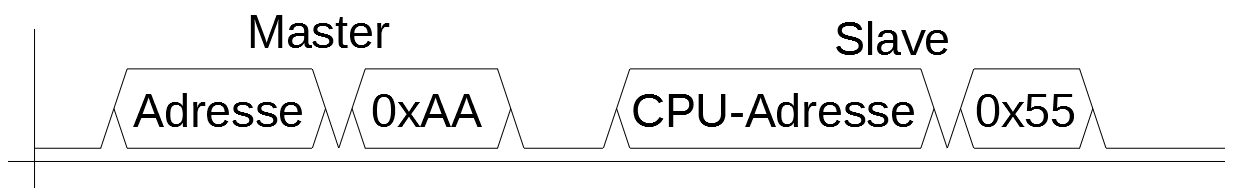
\includegraphics[width=\textwidth]{pictures/ping_protocol.png}
    \caption{Ping-Befehl}
    \label{img:Ping}
\end{figure}

Sobald der Master mit dem Senden des Befehls fertig ist, muss die Antwort nach spätestens 5ms angekommen sein. Ist dies nicht der Fall, so wird im Error-Register die entsprechende Flag gesetzt und das System geht in die Error-Routine.

\subsubsection{Register Write Byte}
Um ein 8bit-Register zu schreiben, sendet man nach der Slave-Adresse das Command-Byte 0x11, gefolgt von der Registernummer und den Daten. Dabei muss es sich um einen 8bit-Wert handeln. Als Acknowledge sendet der Slave den Wert an die CPU zurück.

\subsubsection{Register Write Word}
Um ein 16bit-Register zu schreiben, sendet man nach der Slave-Adresse das Com-mand-Byte 0x12, gefolgt von der Registernummer und den Daten. Dabei muss es sich um einen 16bit-Wert handeln. Als Acknowledge sendet der Slave das Low-Byte an die CPU zurück.

\subsubsection{Register Write Block}
Um mehrere aufeinanderfolgende register zu schreiben, sendet man nach der Slave-Adresse das Command-Byte 0x13, gefolgt von dem Start-Register und den Daten. Dabei werden die High-Bytes stehts zuerst gesendet, sollte es sich um Wörter statt Bytes handeln. Als Acknowledge sendet der Slave die Anzahl an Bytes, die geschrieben wurden, zurück.

Sollte der Slave nicht in der Lage sein, alle Bytes in Register zu schreiben, so werden die Register gefüllt und nachfolgende Bytes verworfen. Sobald der Master aufgehört hat zu senden, meldet der Slave den Error-Code 0xF1 an die CPU zurück.

\subsubsection{Register Read Byte}
Um ein 8bit-Register zu lesen, sendet man nach der Slave-Adresse das Command-Byte 0x21, gefolgt von der Registernummer. Der Slave antwortet nach 1ms mit dem Wert des Registers. Ein Acknowledge von Seiten der CPU gibt es nicht. 

Sollte es dem Slave nicht möglich sein, aus dieser Registernummer zu lesen, so sendet er die Daten 0xDEAD

\subsubsection{Register Read Word}
Um ein 16bit-Register zu lesen, sendet man nach der Slave-Adresse das Command-Byte 0x22, gefolgt von der Registernummer. Der Slave antwortet nach 1ms mit dem Wert des Registers. Ein Acknowledge von Seiten der CPU gibt es nicht. 

Sollte es dem Slave nicht möglich sein, aus dieser Registernummer zu lesen, so sendet er die Daten 0xFDEADF				\newpage	% Bus Erklärung



	

% --------------------------------------------------------------------
% abschließende Verzeichnisse
% --------------------------------------------------------------------

\pagestyle{empty}
\vspace*{\fill}
\begin{center}
\hrulefill\\
\vspace{4mm}
	\begin{HUGE}
		\textbf{ANHANG}
	\end{HUGE}\\
\hrulefill
\end{center}
\vspace*{\fill}
\newpage
\pagestyle{plain}


\appendix

% --------------------------------------------------------------------
\end{document}
